\section{Gráficas de robot 1:}
\vspace{10mm}

ROBOT A)
\vspace{10mm}

 Solución alcanzada en muestra 1, iteraciones 6, error = 1.012130e-07

 Solución alcanzada en muestra 1, iteraciones 6, error = 5.542149e-08

\vspace{10mm}

\begin{figure}[h]
	\centering
	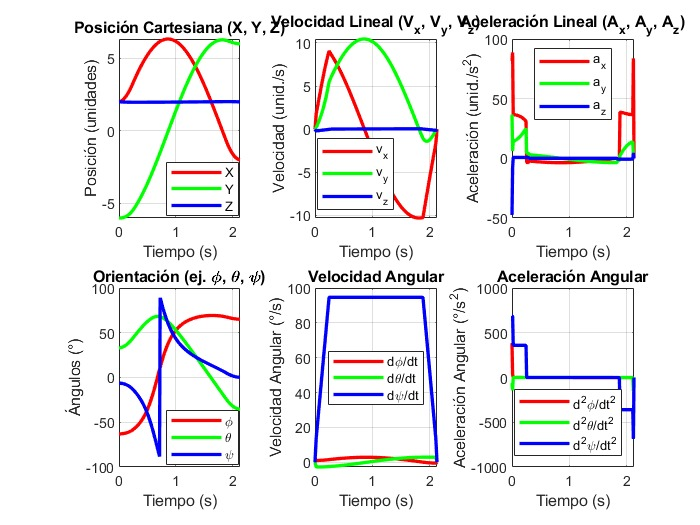
\includegraphics[width=0.55\linewidth]{img/R1}
	\caption{}
	\label{fig}
\end{figure}

\begin{figure}[h]
	\centering
	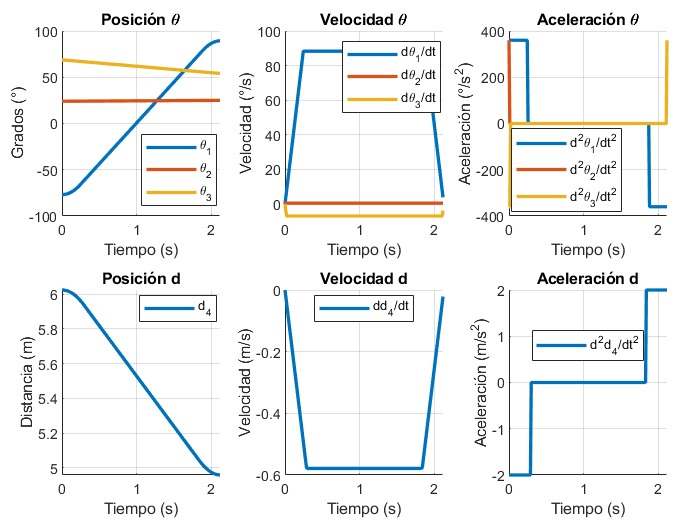
\includegraphics[width=0.55\linewidth]{img/R1 2}
	\caption{}
	\label{fig}
\end{figure}

% Espacio para evitar que LaTeX mueva imágenes
\vspace{5mm}

\newpage  % Salto de página forzado
\vspace{10mm}

ROBOT B)
\vspace{10mm}

Solución alcanzada en muestra 1, iteraciones 6, error = 8.703720e-07

Solución alcanzada en muestra 1, iteraciones 6, error = 3.678459e-10


\vspace{10mm}

\begin{figure}[h]
	\centering
	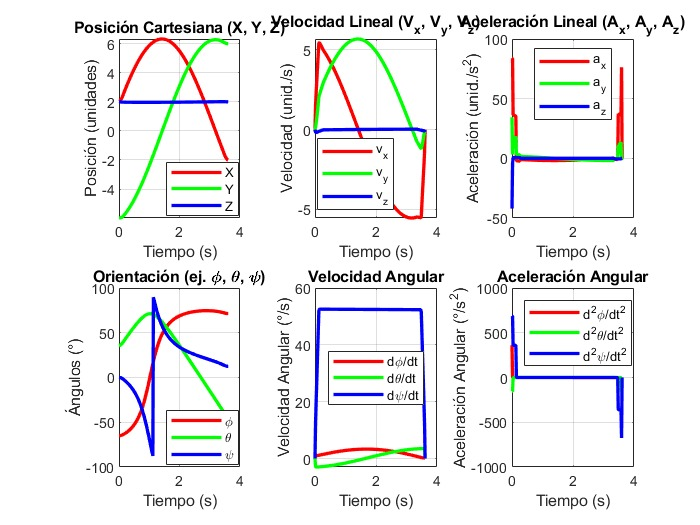
\includegraphics[width=0.6\linewidth]{img/R2}
	\caption{}
	\label{fig}
\end{figure}

\begin{figure}[h]
	\centering
	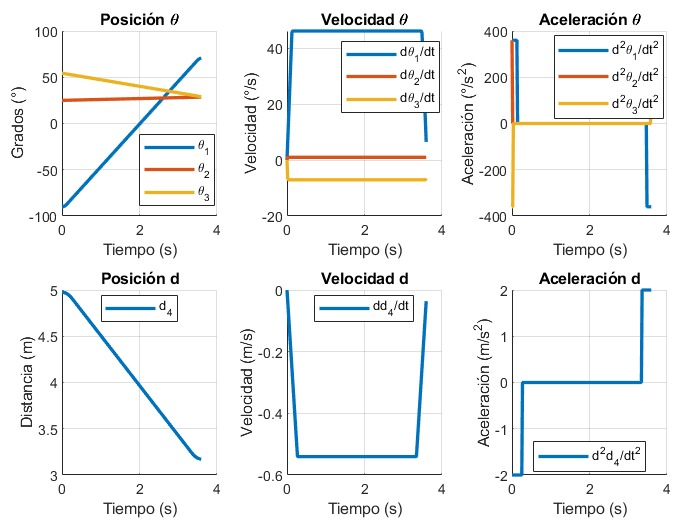
\includegraphics[width=0.6\linewidth]{img/R2 2}
	\caption{}
	\label{fig}
\end{figure}

% Espacio para evitar que LaTeX mueva imágenes
\vspace{5mm}